\section{Desired properties of training data}
\label{sec:desiredpropdata}
\begin{figure*}[!htb]
\centering
\begin{tabular}{c}
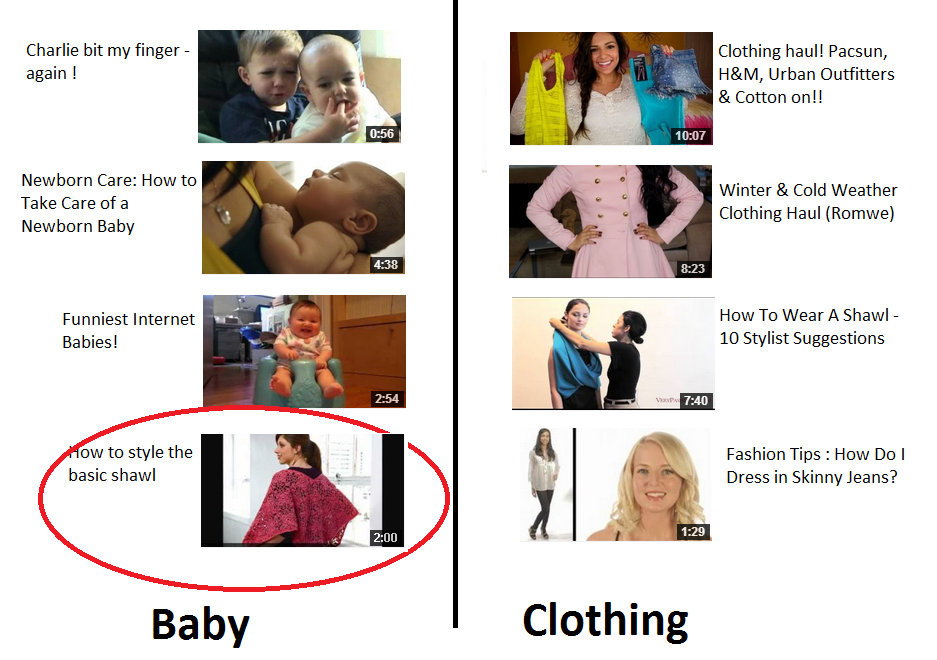
\includegraphics[width=0.45\textwidth,clip=]{TrainingData/WIfigures/mislabeled_baby_clothes_marked.png}
 \\
(a) \\ \\ 
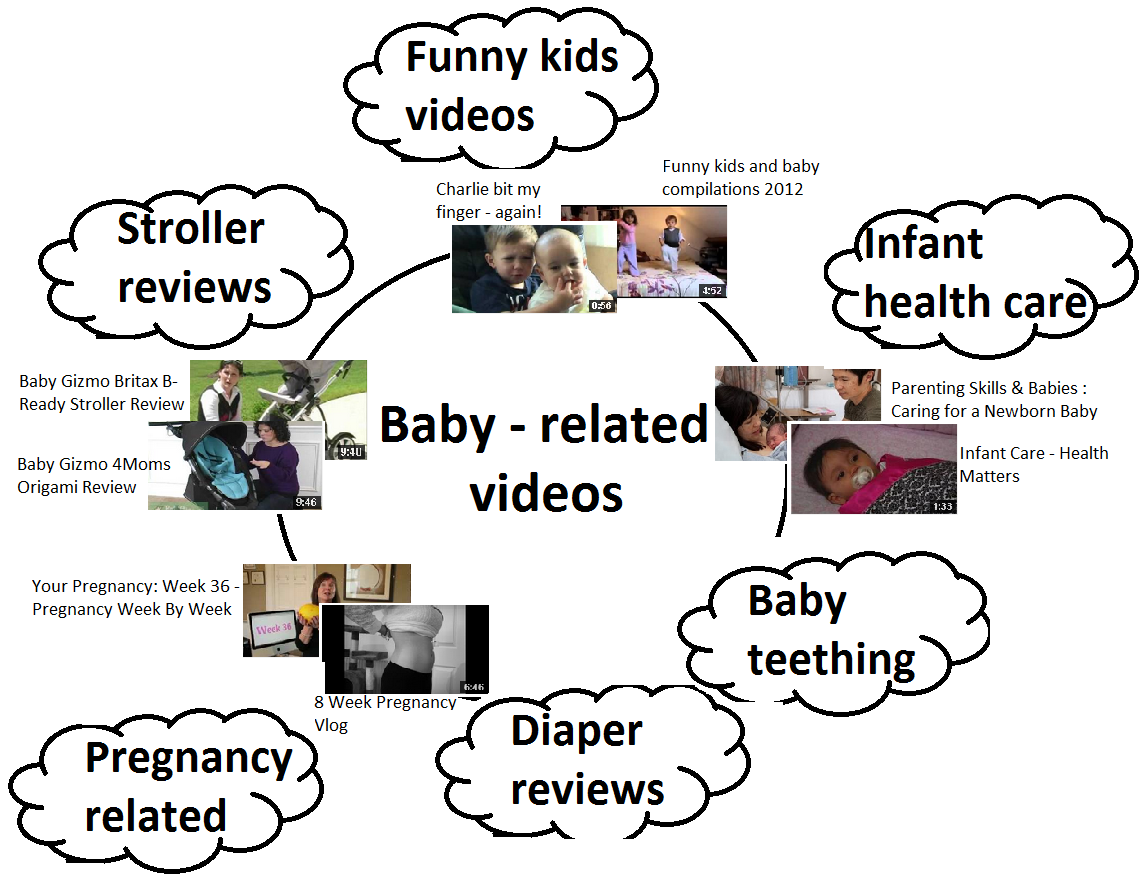
\includegraphics[width=0.45\textwidth,clip=]{TrainingData/WIfigures/diversity_baby5.png} \\ 
(b) \\ 
\end{tabular}
\caption{ \small{(a) Sample training videos for categories: \{\textit{Baby, Clothing}\}. Circled video is wrongly placed in category $Baby$, and is hence a mislabeled video. (b) Variety of video topics belonging to category $Baby$  }}
\label{fig:trainingdatapropsfigs}
\end{figure*} 
For a given classification model, a good training data would be one that has no mislabeled instances, and has high Intra-Category Diversity for each category. We discuss both factors in this section. The goodness of training data is reflected in terms of its performance on a large test set. 

In the domain of video classification, a mislabeled instance refers to a video that has the label of category $i$ as per the training data, but in actual, belong to a different category $j ( \neq i)$ as per an oracle. For instance, consider the set of categories \{\textit{Baby, Clothing, Fitness, Food}\} that a retailer may be interested in, to enable personalized promotions of the above product categories. If certain approach for obtaining training videos includes a video on $Shawls$ (as shown in Fig.~\ref{fig:trainingdatapropsfigs}(a)) to the set of training videos for $Baby$, the video would be a mislabeled video since its true label should be $Clothing$, but it has the label of $Baby$ in training data. A true label of a video is defined as the label that an oracle would assign to the video. \cite{brodley1996identifying,zhu2003eliminating} discuss techniques to identify (and eliminate) mislabeled instances from training data, for classification tasks. The performance of classification models is shown to have increased considerably after identifying (or eliminating) mislabeled videos, thus supporting that less mislabeled instances is desired in training data.  Note that the above works address the cleaning of an existing dataset whereas the problem addressed in this chapter is that of \textit{forming} a dataset by obtaining training videos with desired properties for certain given categories. In addition, in works such as \cite{brodley1996identifying} and \cite{zhu2003eliminating}, the mislabeled instances are identified as outliers in the given data, when the data itself is representative of the class in concern and captures its constituent topics. While forming a training data from real world videos retrieved using keywords, this condition is not guaranteed to be satisfied and the above techniques may not be applied. These techniques can be considered orthogonal to our work, and may further improve the training data \textit{after} it is formed using the proposed framework. 

By Intra-Category Diversity of training videos $T(i)$ of category $i$, we refer to the extent to which $T(i)$ encompasses the essence of category $i$. Let us denote Intra-Category Diversity of $T(i)$ as $div(T(i))$. In order to first intuitively motivate why high $div(T(i))$ is desired, consider the same set of categories \{\textit{Baby, Clothing, Fitness, Food}\}. Fig.~\ref{fig:trainingdatapropsfigs}(b) shows some of the various topics of videos that one would associate with the category $Baby$. A set of training videos $T_1$, having videos on \textit{Funny kids} only has less Intra-Category Diversity than a set $T_2$ of same cardinality as $T_1$ but having videos on \textit{Funny kids, Newborn care, Babysitting}, and \textit{Stroller reviews}. A classifier trained over $T_2$ is expected to have higher likelihood of categorizing correctly a test video $v$ belonging to category Baby as compared to a classifier trained over $T_1$. For instance, if a user watches a video related to review of popular strollers for infants, the model trained on $T_2$ will find it more similar to the training videos on $Baby$ than the model trained on $T_1$ will, and hence will have higher likelihood of categorizing it correctly. 

As discussed later in Section~\ref{sec:overview}, one of the shortcomings of approaches that obtain training videos without manual labeling is low Intra-Category Diversity. In such scenario, the training data of a category is skewed towards certain dominant themes within the category, and encompasses only limited topics of videos within the category. Improved techniques are hence required to obtain training videos with high Intra-Category Diversity. While it is understandable what $div(T(i))$ means, calculation of $div(T(i))$ requires knowledge of a) different topics within category $i$, and b) the extent to which these topics are covered by the training videos of category $i$. For an arbitrary set of categories, it is extremely difficult to obtain (a) and (b) above without the help of an oracle. Thus in our research, we propose the use of different techniques to obtain the degree of variation in $T(i)$ to measure $div(T(i))$. These techniques are discussed in Section~\ref{sec:overview}, and their details are provided with the respective approaches (Sections~\ref{sec:lcpd} and \ref{sec:aao}). 

The notion of diversity has been used for a variety of problems in related domains. Diversity between classification models has been discussed in works on classification model ensembles \cite{Ludmila03}. Works on summarization have used the notion of diversity between documents \cite{LiEnhanc09,ZhuNovSum13}, images \cite{KennedyGen08} and videos \cite{ShroffTMM10}. In the context of active learning \cite{WangActive11} and semi-supervised learning \cite{MisraWatch15}, diversity has been used to efficiently determine training instances to label manually. To the best of our knowledge, the use of diversity metrics in the formulation to automatically obtain training videos for classification is completely novel. 

%In Section~\ref{sec:selectionSRK}, we present numerical values for the Intra-Category Diversity and experimentally verify that an increase in Intra-Category Diversity of training data translates to improved performance of the trained classifier. 